\subsection{If a parent class imports a class from different package, the target child class within same java file cannot be duplicate with that imported class after rename.}

If a parent class imports a class from different package and if we try renaming a child class with the same name as the class imported into its parent class within the same java file, compiler produces the error as `a compilation unit must not import and declare a type with the same name'~\cite{EclipseWebPage}.This precondition can be explained by the following example.

\begin{figure}[th]
\centering
\begin{minipage}[t]{0.45\linewidth}
\begin{lstlisting}[language=java, basicstyle=\scriptsize\ttfamily,frame=single]	
A.java

package q;
import p.C;
class A{	
}
class B extends A{	
}
class D extends B{
}
\end{lstlisting}
\tiny{(a) Before renaming Subclass B}
\end{minipage}
\hfill
\begin{minipage}[t]{0.45\linewidth}
\begin{lstlisting}[language=java, basicstyle=\scriptsize\ttfamily,frame=single]
A.java

package q;
import p.C;
class A{	
}
class C extends A{	
}
class D extends B{
}	
\end{lstlisting}
\tiny{(b) After Renaming Child class  B to C}
\end{minipage}
\caption{Precondition for Renaming Child class within the same java file}
\label{figure:fig7}
\end{figure}

From the above figure \ref{figure:fig7}, We see that if one has imported class C from  package  p to the parent Class A and if we try to rename the child class B to C or D to C, Compiler produces  the error as given in the figure \ref{figure:fig8}. As mentioned in  section \ref{sec:precon2}, the same precondition also holds good for renaming a sub-class. This precondition is applicable for all ancestor class, so one has to trace back and check if any of the parent class is importing a class with same name before renaming the child class within the same java file.
\begin{figure}[htbp]
\centerline{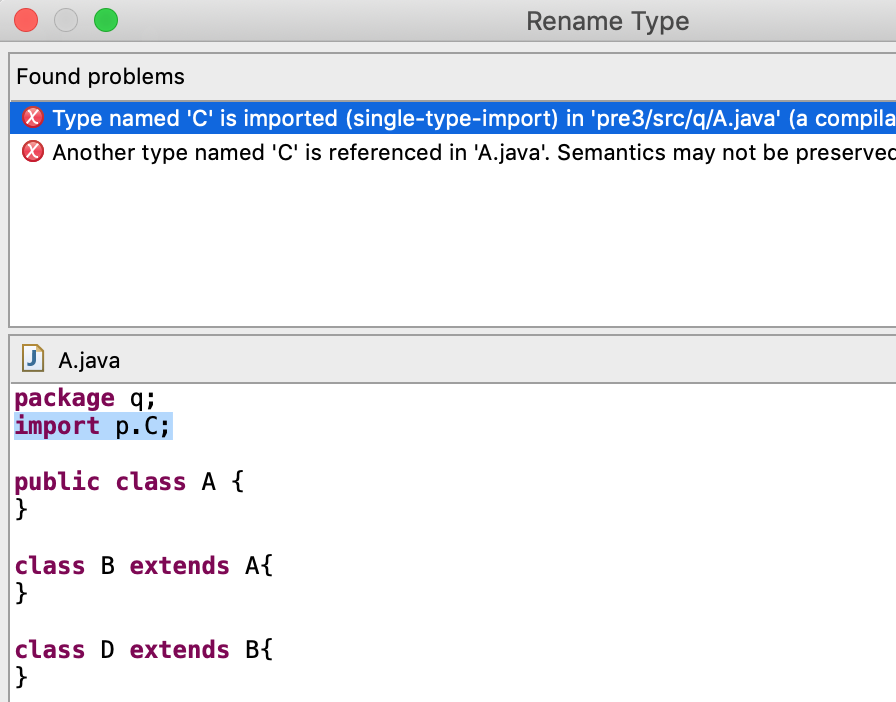
\includegraphics[width=85mm,scale=0.5]{precond3.png}}
\caption{Error produced after renaming the sub-class.}
\label{figure:fig8}
\end{figure}

If a parent class imports a class from different package and if the child class is defined in a separate java file. At that time we can refactor and rename the child class to the imported class name.
In the below figure \ref{figure:fig8}, We see that child class of B (class D)is defined in separate java file and this time we can easily refactor and rename the child class D to C.
\begin{figure}[th]
\centering
\begin{minipage}[t]{0.45\linewidth}
\begin{lstlisting}[language=java, basicstyle=\scriptsize\ttfamily,frame=single]	
A.java

package q;
import p.C;
class A{	
}
class B extends A{	
}

D.java

class D extends B{
}
\end{lstlisting}
\tiny{(a) Before renaming Child class D}
\end{minipage}
\hfill
\begin{minipage}[t]{0.45\linewidth}
\begin{lstlisting}[language=java, basicstyle=\scriptsize\ttfamily,frame=single]
A.java

package q;
import p.C;
class A{	
}
class B extends A{	
}

C.java

class C extends B{
}	
\end{lstlisting}
\tiny{(b) After Renaming Child Class D to C}
\end{minipage}
\caption{Precondition for Renaming Child Class in separate java file}
\label{figure:fig8}
\end{figure}